% !TEX TS-program = xelatex
% !TEX encoding = UTF-8
% !Mode:: "TeX:UTF-8"

\documentclass[onecolumn,oneside]{SUSTechHomework}

\usepackage{blindtext}
\usepackage{graphicx}
\usepackage{subfigure}
\usepackage{float}
\usepackage{listings}
\usepackage{hyperref}
\usepackage{framed}
\usepackage{extarrows}
\usepackage{algorithm}
\usepackage{algorithmic}
\hypersetup{hidelinks,
	colorlinks=true,
	allcolors=black,
	pdfstartview=Fit,
	breaklinks=true}

\begin{document}
\author{任振裕}
\sid{11812214}
\title{Laboratory 5: Fast Fourier Transform}
\coursecode{EE323}
\coursename{Digital Signal Processing}
\date{November 26, 2020}
\maketitle

\section*{5.1 Introduction}
The last laboratory covers the Discrete Fourier Transform (DFT). This laboratory will continue the
discussion of the DFT and will introduce the Fast Fourier Transform(FFT). This lab will mainly contain
the flowing contents:
\begin{itemize}
    \item Continuation of DFT Analysis
    \item The Fast Fourier Transform Algorithm
    \item My explorations for FFT Algorithm
\end{itemize}
Through this lab, we could have a deeper understanding of principles of FFT algorithm. In 
order to show the advantages of FFT, we also involve the computational complexity to make 
a comparison between the conventional DFT calculated method (DFTsum in the previous lab) and FFT
method. 

\section*{5.2 Continuation of DFT Analysis}
\subsection*{5.2.1 Shifting the Frequency Range}
\subsubsection*{A. Plot of magnitude of $|X_{20}[k]|$ versus $k$ (DFTsum of hamming window with $N=20$).}
\begin{itemize}
	\item MATLAB codes:
\begin{lstlisting}[title=\textbf{q5\_2\_1.m}]
	clear;
	% part 1
	N = 20;
	k = 0:N-1;
	x = hamming(20);
	X20 = DFTsum(x);
	figure(1);
	stem(k,abs(X20)),xlabel('k'),ylabel('magnitude of |X_{20}[k]|'),title('magnitude of |X_{20}[k]|');
	xlim([-1,20]);ylim([-2,max(abs(X20))+2]);
	% part 2
	figure(2);
	[X,w] = DTFTsamples(x);
	figure(2);
	stem(w,abs(X)),xlabel('\omega(rad/sample)'),ylabel('magnitude of DTFT samples of x[n]'),title('magnitude of DTFT samples of x[n]');
	xlim([w(1)-0.1,w(N)+0.1]);ylim([-2,max(abs(X))+2]);
\end{lstlisting}
	\item Running Result:
\begin{figure}[H]
	\centering
	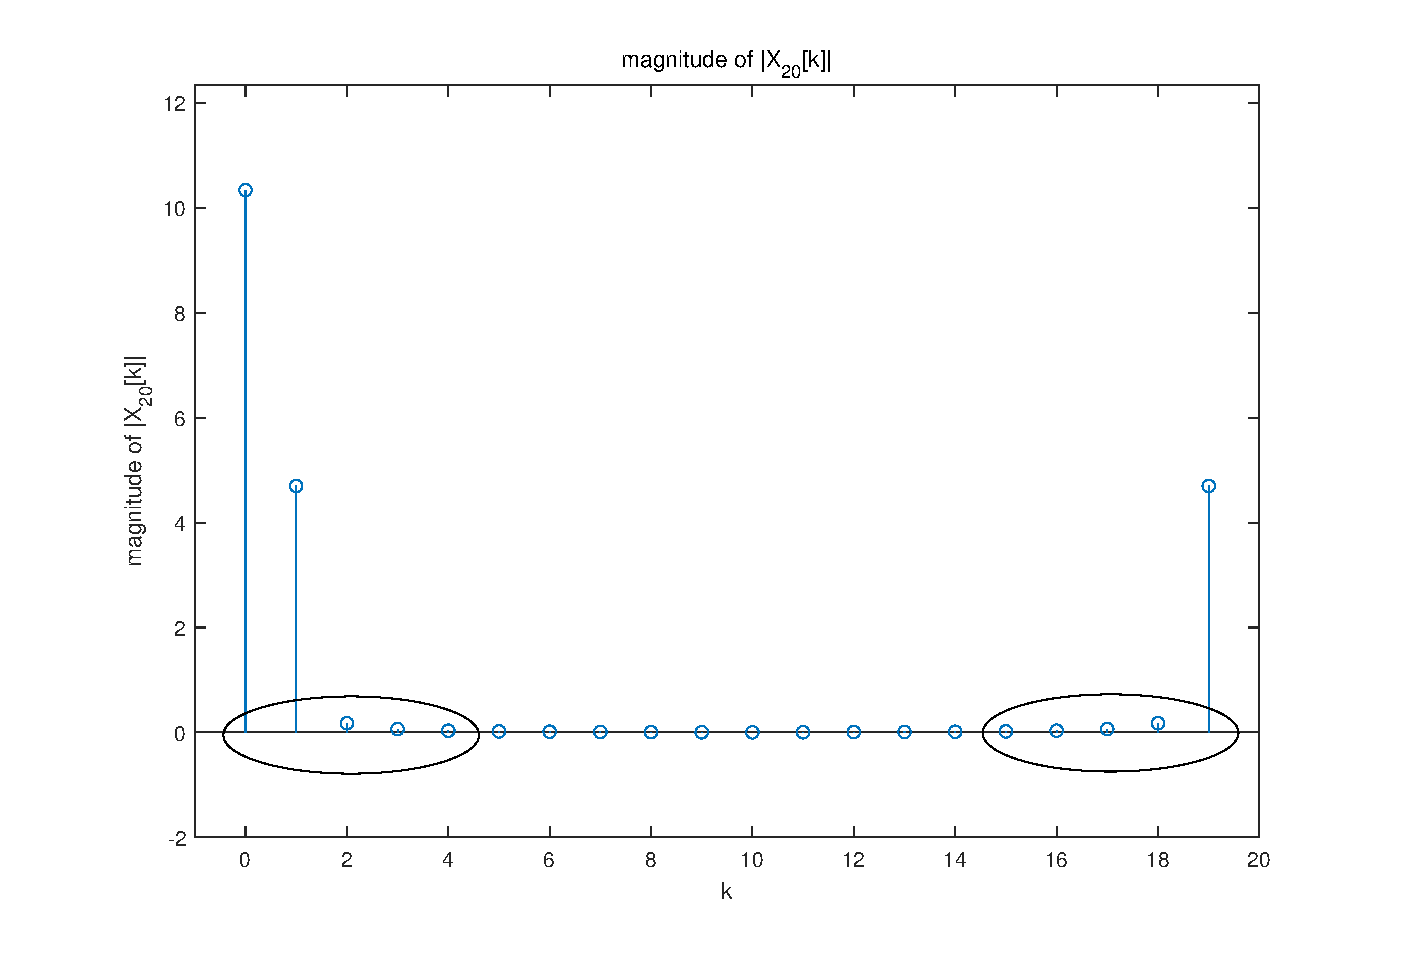
\includegraphics[width=150mm]{pictures/X20k.eps}
	\caption{Plot of magnitude of $|X_{20}[k]|$ versus $k$}
\end{figure}
	\item Analysis:
	\begin{itemize}
		\item The regions of low frequency component is shown in the circles of above figures;
		\item There are two disadvantages of this plot:
		\begin{enumerate}
			\item The plot is against $k$ rather than $\omega$.
			\item The arrangement of frequency samples goes against $[0,2\pi]$ rather than $[-\pi,\pi]$.
		\end{enumerate}
	\end{itemize}
\end{itemize}
\subsubsection*{B. Plot of DTFTsamples.}
\begin{itemize}
	\item MATLAB codes for \textbf{DTFTsamples.m}:
\begin{lstlisting}[title=\textbf{DTFTsamples.m}]
	function [X,w] = DTFTsamples(x)
	N = length(x);
	k = 0:N-1;
	w = 2*pi*k/N;
	w(w>=pi)=w(w>=pi)-2*pi;% shift the range from [0,2*pi] to [-pi,pi]
	w = fftshift(w);
	X = fftshift(DFTsum(x));
	display(w);display(X);
	end 
\end{lstlisting}
	\item Plot of DTFTsamples of hamming window with $N=20$.
\begin{figure}[H]
	\centering
	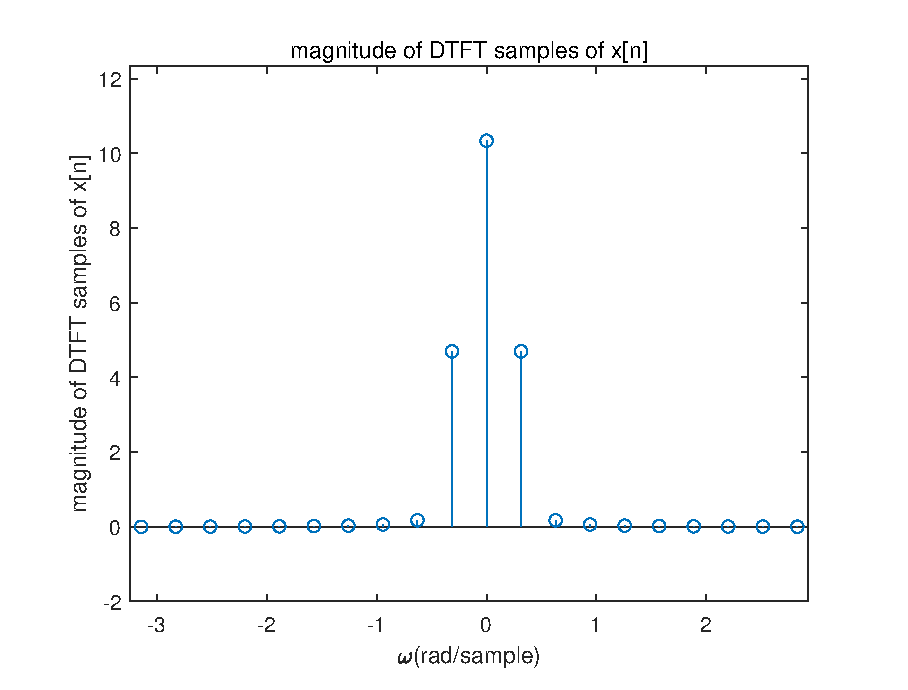
\includegraphics[width=150mm]{pictures/fig2.eps}
	\caption{Plot of DTFTsamples of hamming window with $N=20$}
\end{figure}
	\item Analysis: 
	\begin{itemize}
		\item By applying the DTFTsamples ($\omega=2\pi k/N$), the plot is against $\omega$ now.
		\item By applying the algorithm of \textbf{fftshift()} for both $\omega$ and DTFTsamples,
		we could achieve the arrangement of frequency goes against $[-\pi,\pi]$.
	\end{itemize}
\end{itemize}
\subsection*{5.2.2 Zero Padding}
\begin{itemize}
	\item Finite duration signal considered in this section:
$$
x[n]=\begin{cases}
	\ \sin (0.1 \pi n), & 0 \leq n \leq 49\\
	\ 0, & \text{otherwise} 
\end{cases}
$$
$$
\text{length}(x[n])=N
$$
	\item MATLAB codes for this section:
\begin{lstlisting}[title=\textbf{q5\_2\_2.m}]
	clear;
	x = sin(0.1*pi*[0:49]);
	N = input("Please specify a range N:\n");
	display(N);
	x = [x zeros(1,N-50)];% zero padding;
	display(x)
	[X,w] = DTFTsamples(x);
	stem(w,abs(X)),xlabel('\omega(rad/sample)'),ylabel('magnitude of DTFT samples of x[n]'),title('magnitude of DTFT samples of x[n]');
\end{lstlisting}
	\item Plot of DTFTsamples when $N=50$ (No zero paddings):
\begin{figure}[H]
	\centering
	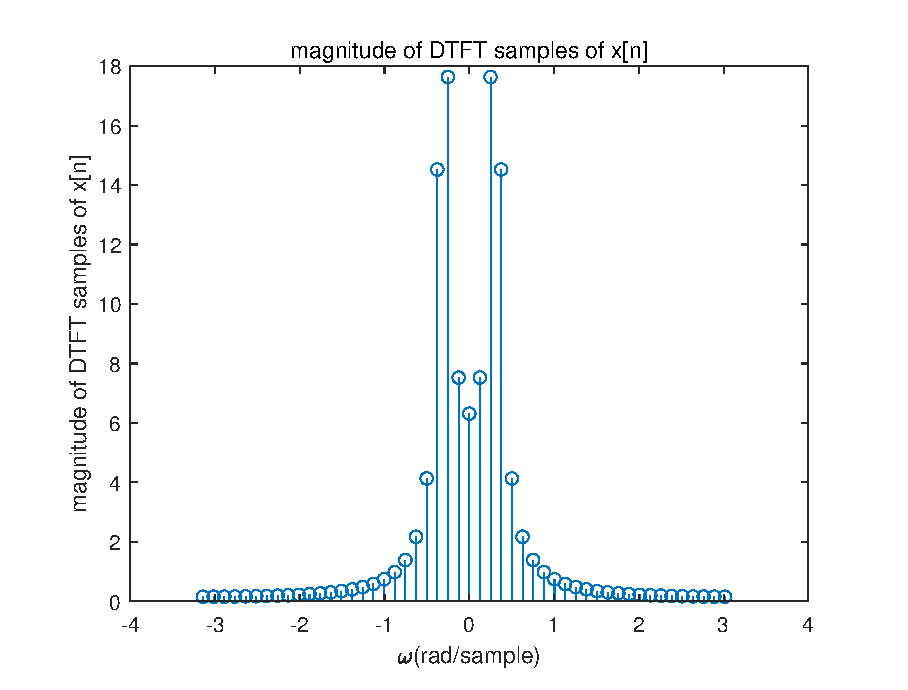
\includegraphics[width=135mm]{pictures/q5_2_2_N50.eps}
	\caption{Plot of DTFTsamples when $N=50$}
\end{figure}
	\item Plot of DTFTsamples when $N=200$:
\begin{figure}[H]
	\centering
	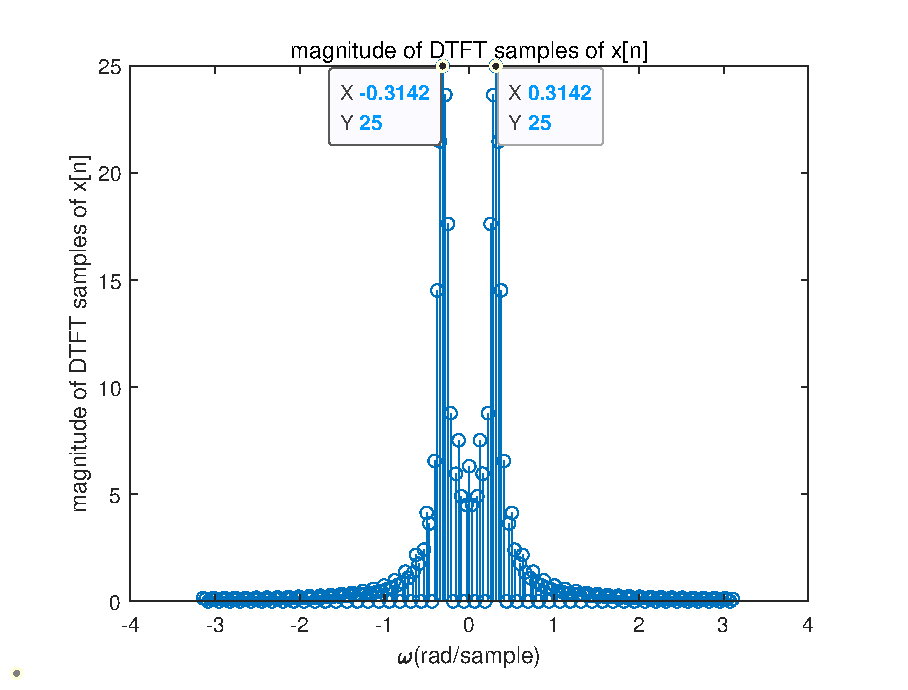
\includegraphics[width=135mm]{pictures/q5_2_2_N200.eps}
	\caption{Plot of DTFTsamples when $N=200$}
\end{figure}
	\item Analysis: Evidently, graph of case $N=200$ looks more like DTFT than case $N=50$.
	\item Proof (Why is case $N=200$ closer to DTFT?): 
		\begin{itemize}
			\item Shape of truncated signal $x[n]=\sin (0.1\pi n), 0 \leq n \leq 49$ 's DTFT: \par
			Evidently, $x[n]$ is a truncated signal truncated by sine function $x'[n]=\sin (0.1\pi n), -\infty<n<\infty$ 
			with window function $\omega[n]=1, 0 \leq n \leq 49$. \par
			It has been shown in the previous laboratory that truncated signal's DTFT has below forms:
			$$
			\begin{aligned}
				X(e^{j\omega})&=Ft\{x[n]\times w[n]\}\\
				&=X'(e^{j\omega})\circledast W(e^{j\omega})\\
				&=(\pi\delta(\omega-0.1\pi)+\pi\delta(\omega+0.1\pi))\circledast W(e^{j\omega})\\
				&=\pi W(e^{j(\omega-0.1\pi)})+\pi W(e^{j(\omega+0.1\pi)})
			\end{aligned}
			$$
			Where, $W(e^{j\omega})$ is a sinc wave such that:
			$$
			\begin{aligned}W\left(e^{j \omega}\right) &=\sum_{n=-\infty}^{\infty} w[n] e^{-j \omega n}=\sum_{n=0}^{N-1} e^{-j \omega n} \\
				&=\left\{\begin{array}{ll}\frac{1-e^{-j \omega N}}{1-e^{-j \omega}}, & \text { for } \omega \neq 0, \pm 2 \pi, \ldots 
					\\N, & \text { for } \omega=0, \pm 2 \pi, \ldots\end{array}\right.
			\end{aligned}
			$$
			$$
			W\left(e^{j \omega}\right)=\frac{e^{-j \omega N / 2}}{e^{-j \omega / 2}} \frac{e^{j \omega N / 2}-e^{-j \omega N / 2}}{e^{j \omega / 2}-e^{-j \omega / 2}}
			=e^{-j \omega(N-1) / 2} \frac{\sin (\omega N / 2)}{\sin (\omega / 2)}
			$$
			$\therefore$ DTFT waveform of $x[n]$ is composed of two sinc function centered at $-0.1\pi$ and $0.1\pi$ respectively.
			\item Already known the waveform of DTFT, let us pay attention to the Figure 3 and Figure 4:\par
			Evidently, Figure 4 provides closer waveform to sinc waveforms. And the center of waveform shown in
			Figure 4 (0.3142 and -0.3142) just satisfy the previous deduction that two sinc waves centered at $-0.1\pi$ and $0.1\pi$.
		\end{itemize}
		\item Why these two plots look so differently?
		\begin{itemize}
			\item This is just because of effects of zero-paddings. The more padding zeros there are, the closer to
			DTFT waveform of DFT is.
			\item Proof: Just take a look into the equation of DTFT and DFT:\par
			DTFT:
			$$
			X(e^{j\omega})=\sum_{n=-\infty}^{\infty}x[n]e^{-j\omega n}
			$$
			DFT:
			$$
			X_N[k]=\sum_{n=0}^{N-1}x_N[K]e^{j2\pi kn/N}
			$$
			It could be observed that DFT is frequency sampling of DTFT at $\omega=2\pi k/N, k=0,1,...,N-1$.\par
			$\therefore$ Case $N=200$ provides smaller sampling interval than case $N=50$.\par
			$\therefore$ These two cases look different and case $N=200$ is closer to DTFT.
		\end{itemize}         
\end{itemize}
\section*{5.3 The Fast Fourier Transform Algorithm}
\subsection*{5.3.1 Implementation of Divide-and-Conquer DFT}
\begin{itemize}
	\item Diagram of Figure dcDFT. (Only consider N/2 points dcDFT)
	\begin{figure}[H]
		\centering
		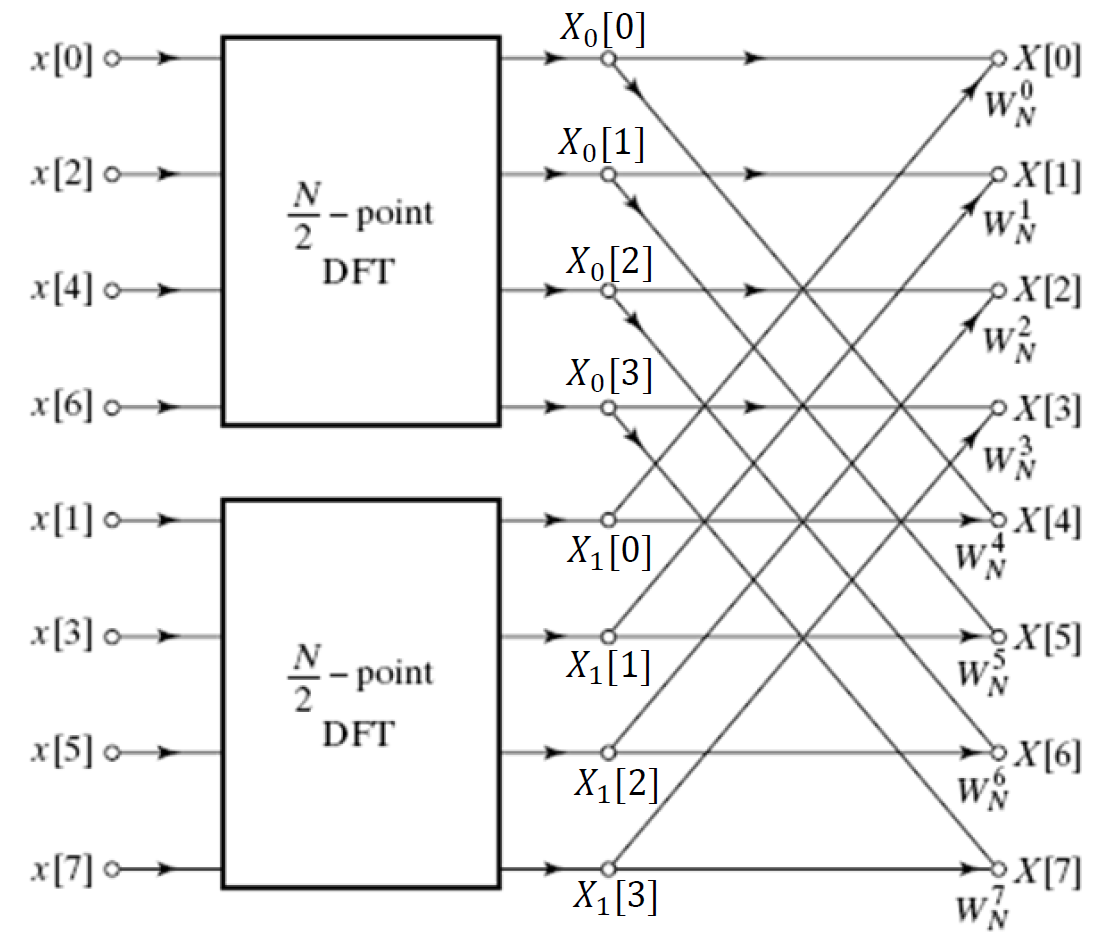
\includegraphics[width=130mm]{pictures/dcDFT.png}
		\caption{Diagram of dcDFT}
	\end{figure}
	Figure 5 could be described as below equation:
	\begin{equation}
		X[k]=X_{0}\left[\langle k\rangle_{N / 2}\right]+W_{N}^{k} X_{1}\left[\langle k\rangle_{N / 2}\right] \tag{Strategy 1}
	\end{equation}
	Where, $k=0,1,...,N-1 $.
	\item MATLAB code for \textbf{dcDFT.m}:
\begin{lstlisting}[title=\textbf{dcDFT.m}]
	function X = dcDFT(x)
	% Using divide and conquer method to calculate FFT
	% 2 stages of FFT only, computational complexity: N+N^2/2
	% Divide the input into even and odd parts
	N = length(x);  % Even length N
	x0 = x(1:2:N);  % Even part of x[n]: x[0],x[2],...,x[N-2]
	x1 = x(2:2:N);  % Odd part of x[n]: x[1],x[3],...,x[N-1]
	X0 = DFTsum(x0); X0 =[X0 X0];
	X1 = DFTsum(x1); X1 = [X1 X1];
	X = X0+ exp(-j*2*pi/N*[0:1:N-1]).*X1;
	end
\end{lstlisting}
	\item Verifications for dcDFT: \par
	\begin{itemize}
		\item Test functions:
		\begin{itemize}
			\item $x_1[n]=\delta[n], \text{for}\ N=10$
			\item $x_2[n]=1, \text{for}\ N=10$
			\item $x_3[n]=e^{j2\pi n/N}, \text{for}\ N=10$
		\end{itemize}
		\item Test codes:
\begin{lstlisting}[title=\textbf{q5\_3\_1}]
	clear;
	n = 0:9; N = length(n);
	x1 = (n==0);
	x2 = ones(1,N);
	x3 = exp(j*2*pi*n/N);
	k = 0:9;
	sgtitle('dcDFT and DFTsum')
	subplot(321),stem(n,abs(dcDFT(x1))),xlabel('k'),ylabel('dcDFT(x1)'),title('magnitude of dcDFT(x1)');
	subplot(322),stem(n,abs(DFTsum(x1))),xlabel('k'),ylabel('DFTsum(x1)'),title('magnitude of DFTsum(x1)');
	subplot(323),stem(n,abs(dcDFT(x2))),xlabel('k'),ylabel('dcDFT(x2)'),title('magnitude of dcDFT(x2)');
	subplot(324),stem(n,abs(DFTsum(x2))),xlabel('k'),ylabel('DFTsum(x2)'),title('magnitude of DFTsum(x2)');
	subplot(325),stem(n,abs(dcDFT(x3))),xlabel('k'),ylabel('dcDFT(x3)'),title('magnitude of dcDFT(x3)');
	subplot(326),stem(n,abs(DFTsum(x3))),xlabel('k'),ylabel('DFTsum(x3)'),title('magnitude of DFTsum(x3)');
\end{lstlisting}	
		\item  Test Result:
		\begin{figure}[H]
			\centering
			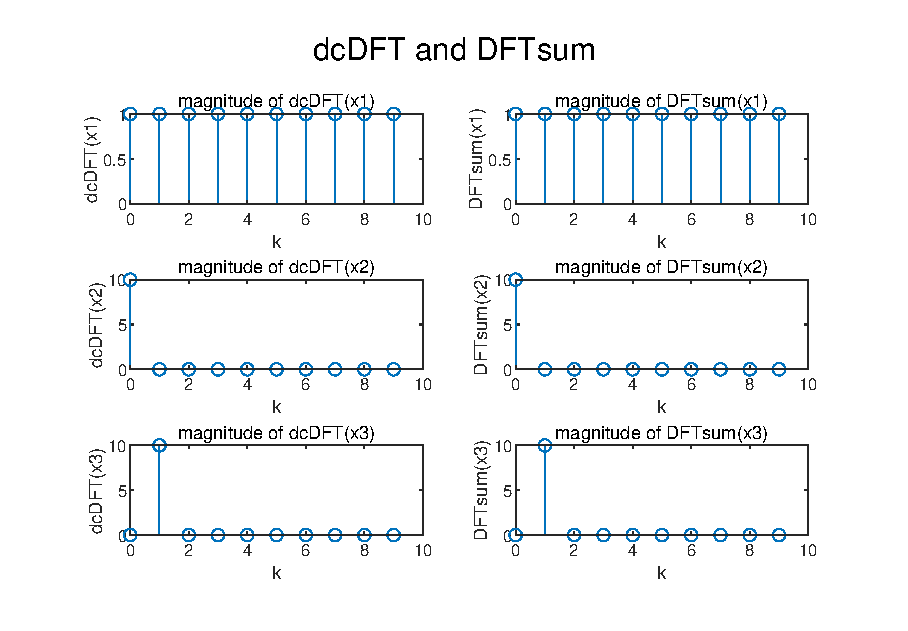
\includegraphics[width=170mm]{pictures/q5_3_1.eps}
			\caption{Verifications for dcDFT}
			(On the left: dcDFT, on the right: DFTsum)
		\end{figure}		 
	\end{itemize}
	\item Analysis: 
	\begin{itemize}
		\item Figure 6 shows that the design of dcDFT is successful.
		\item The number of multiplies that are required in this approach to computing an 𝑁
		point DFT:(Consider a multiply to be one multiplication of real or complex numbers.)
		$$
		N+2\times(N/2)^2=N+N^2/2
		$$
		Proof: According to above Strategy 1, it could be observed that each butterfly needs one multiplication,
		, which could lead to a stage of $N$ points that needs $N$ multiplications. And combining with the condition 
		that $N/2-$points DFTsum operation needs $(N/2)^2$ multiplications, the overall multiplications are $N+2\times(N/2)^2=N+N^2/2$. 
	\end{itemize}
\end{itemize}
\subsection*{5.3.2 Recursive Divide and Conquer}
\subsubsection*{A. 8-point FFT: FFT2,FFT4,FFT8}
\begin{itemize}
	\item Diagram of 8-point FFT:
	\begin{figure}[H]
		\centering
		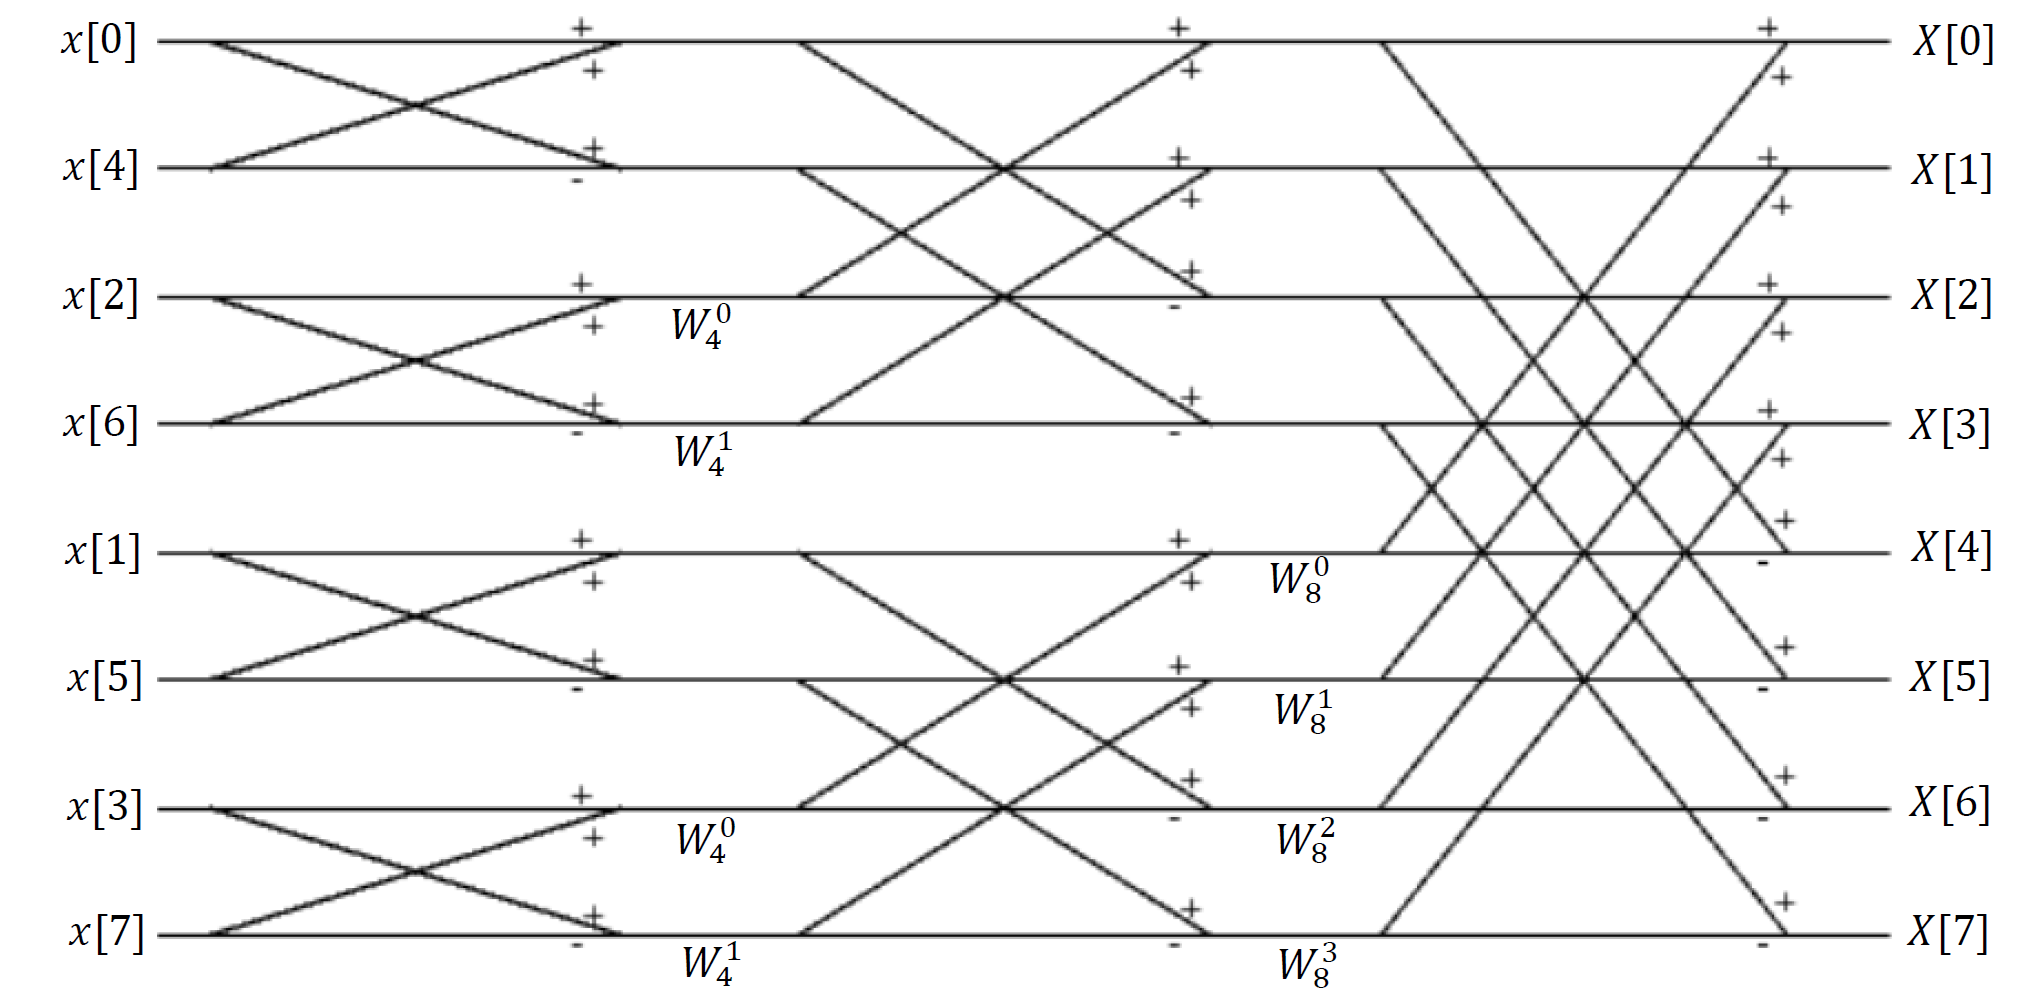
\includegraphics[width=170mm]{pictures/8fft.png}
		\caption{Diagram of 8-point FFT}
	\end{figure}
	\item FFT design strategy in this section:
	\begin{figure}[H]
		\centering
		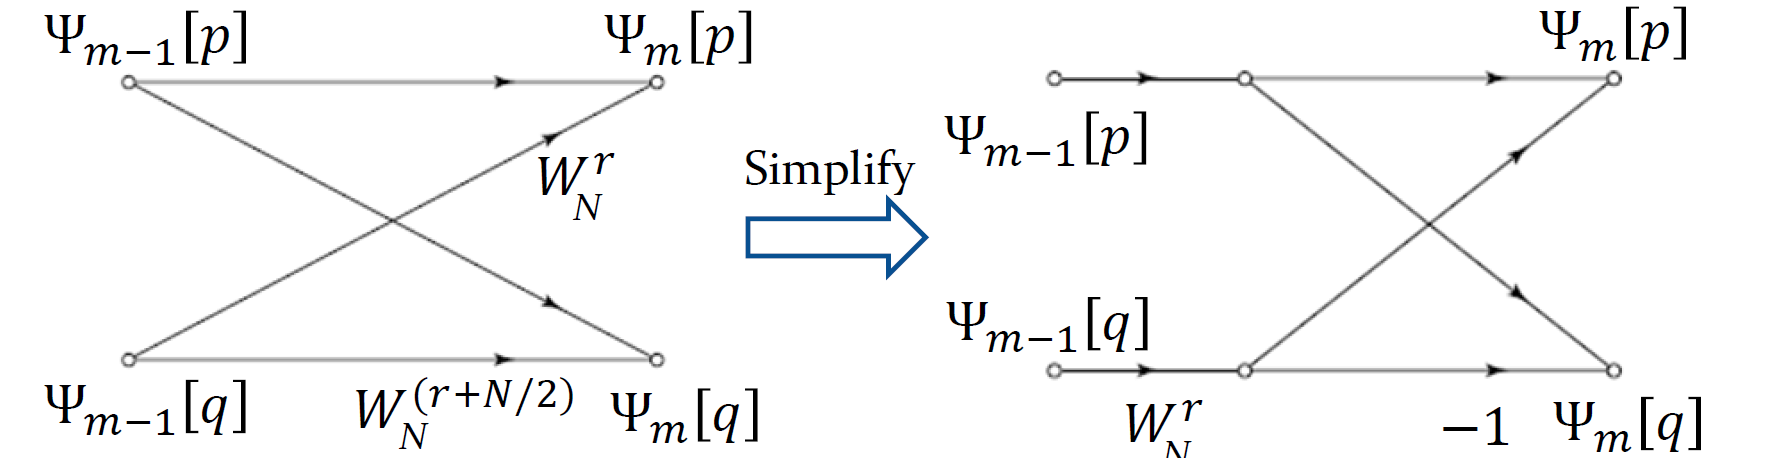
\includegraphics[width=170mm]{pictures/FFT_strategy.png}
		\caption{Simplified butterfly computation}
	\end{figure}
	In this section, we use the below strategy to simplify the calculation of each butterfly.
	\begin{equation}
		\begin{array}{c}\Psi_{m}[p]=\Psi_{m-1}[p]+W_{N}^{r} \Psi_{m-1}[q] 
			\\\Psi_{m}[q]=\Psi_{m-1}[p]+W_{N}^{r+(N / 2)} \Psi_{m-1}[q]=\Psi_{m-1}[p]-W_{N}^r\Psi_{m-1}[q]
		\end{array} \tag{Strategy 2}
	\end{equation}
	By applying such strategy, each butterfly just need one multiplication: $W_{N}^{r} \Psi_{m-1}[q]$.
	Compared with previous Strategy 1, Strategy 2 is much more efficient that each $N-$point stage just needs 
	(N/2) multiplications. 
	\item Three MATLAB functions:
\begin{lstlisting}[title=\textbf{FFT2.m}]
	function X = FFT2(x)
	% length(x) = 2
	X(1) = x(1)+x(2);
	X(2) = x(1)-x(2);
	end		
\end{lstlisting}
\begin{lstlisting}[title=\textbf{FFT4.m}]
	function X = FFT4(x)
	% length(x) = 4
	 r = 0:1;
	 X0 = FFT2([x(1) x(3)]);  
	 X1 = FFT2([x(2) x(4)]); 
	 temp = X1.*exp(-j*2*pi/4*r);
	 X = [X0+temp X0-temp];
	end	
\end{lstlisting}
\begin{lstlisting}[title=\textbf{FFT8.m}]
	function X = FFT8(x)
	% length(x) = 4
	 r = 0:3;
	 X0 = FFT4([x(1) x(3) x(5) x(7)]);
	 X1 = FFT4([x(2) x(4) x(6) x(8)]); 
	 temp = X1.*exp(-j*2*pi/8*r);
	 X = [X0+temp X0-temp];
	end
\end{lstlisting}
	\item Output of \textbf{FFT8} for the case $x[n]=1,\ \text{for}\ N=8$:
	\begin{center}
		\fcolorbox{black}{gray!5}{
			\parbox{1\linewidth}{
				>> FFT8(ones(1,8))
				
				ans =
				
					 8     0     0     0     0     0     0     0
				
				>> fft(ones(1,8))==FFT8(ones(1,8))
				
				ans =
				
				  1$\times$8 logical 数组
				
				   1   1   1   1   1   1   1   1
			}
		}
	\end{center}
	\item Other test examples:($x[n]=\delta[n]$ and $x[n]=e^{\frac{j2\pi n}{8}}$ for $N=8$.)
	\begin{center}
		\fcolorbox{black}{gray!5}{
			\parbox{1\linewidth}{
				>> FFT8([1 zeros(1,7)])

				ans =
				
					 1     1     1     1     1     1     1     1
				
				>> fft([1 zeros(1,7)])==FFT8([1 zeros(1,7)])
				
				ans =
				
				  1$\times$8 logical 数组
				
				   1   1   1   1   1   1   1   1
			}
		}
	\end{center}
	\begin{center}
		\fcolorbox{black}{gray!5}{
			\parbox{1\linewidth}{
				>> x=exp(j*2*pi/8*[0:1:7]);
				
				>> FFT8(x)
				
				ans =
				
				  -0.0000 + 0.0000i   8.0000 - 0.0000i   0.0000 + 0.0000i   0.0000 + 0.0000i   0.0000 + 0.0000i   0.0000 + 0.0000i   0.0000 + 0.0000i   0.0000 + 0.0000i
				
				>> fft(x)
				
				ans =
				
				  -0.0000 + 0.0000i   8.0000 - 0.0000i   0.0000 + 0.0000i   0.0000 + 0.0000i   0.0000 + 0.0000i  -0.0000 + 0.0000i   0.0000 + 0.0000i   0.0000 + 0.0000i
			}
		}
	\end{center}
	\item Comparison between results obtain from \textbf{DFTsum.m} and \textbf{FFT8.m}:
	\begin{itemize}
		\item $x_1[n]=\delta[n], \text{for}\ N=8$
		\item $x_2[n]=1, \text{for}\ N=8$
		\item $x_3[n]=e^{j2\pi n/N}, \text{for}\ N=8$
		\item Test Codes:
\begin{lstlisting}[title=\textbf{q5\_3\_2a.m}]
	clear
	n=0:1:7;N = length(n);
	x1 = (n==0);
	x2 = ones(1,N);
	x3 = exp(j*2*pi*n/N);
	k = 0:7;
	sgtitle('FFT8 and DFTsum')
	subplot(321),stem(n,abs(FFT8(x1))),xlabel('k'),ylabel('FFT8(x1)'),title('magnitude of FFT8(x1)');
	subplot(322),stem(n,abs(DFTsum(x1))),xlabel('k'),ylabel('DFTsum(x1)'),title('magnitude of DFTsum(x1)');
	subplot(323),stem(n,abs(FFT8(x2))),xlabel('k'),ylabel('FFT8(x2)'),title('magnitude of FFT8(x2)');
	subplot(324),stem(n,abs(DFTsum(x2))),xlabel('k'),ylabel('DFTsum(x2)'),title('magnitude of DFTsum(x2)');
	subplot(325),stem(n,abs(FFT8(x3))),xlabel('k'),ylabel('FFT8(x3)'),title('magnitude of FFT8(x3)');
	subplot(326),stem(n,abs(DFTsum(x3))),xlabel('k'),ylabel('DFTsum(x3)'),title('magnitude of DFTsum(x3)');
\end{lstlisting}
		\item Below result shows that the design of \textbf{FFT8.m} is right.
	\end{itemize}
	\begin{figure}[H]
		\centering
		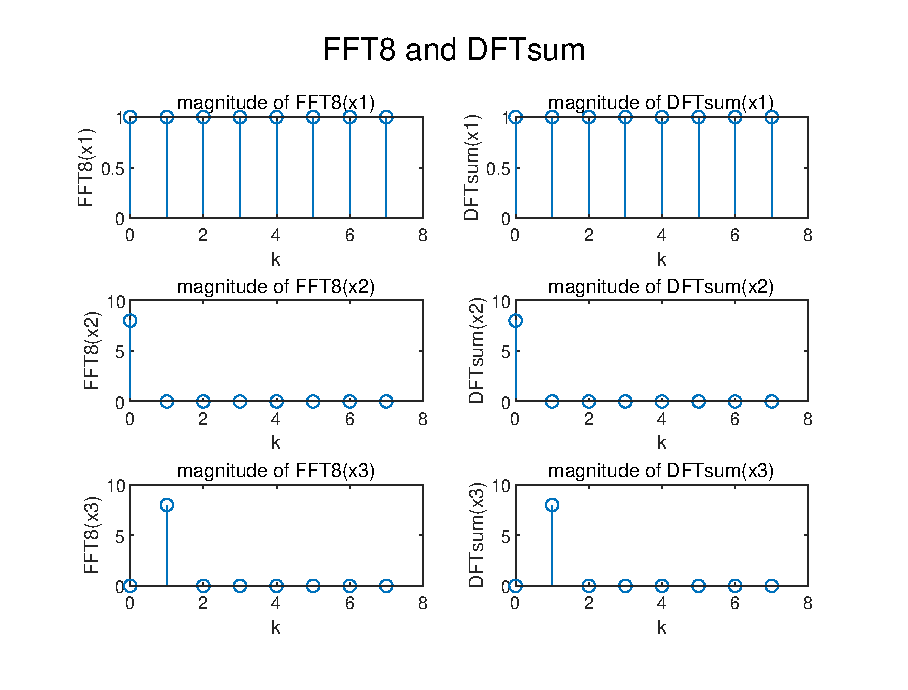
\includegraphics[width=170mm]{pictures/q5_3_2a.eps}
		\caption{Comparison between results obtain from \textbf{DFTsum.m} and \textbf{FFT8.m}}
		(On the right: FFT8, On the left: DFTsum)
	\end{figure}
	\item Analysis: 
	\begin{itemize}
		\item The total number of multiplies by twiddle factors required for 8-point FFT(A multiply is a multiplication by a real or complex number.) : 
		$\frac{8}{2}\times\log_2 8=12$.(Without considering $W_N^0=1$ and $W_N^{N/2}=-1$ in above Strategy 2 here.)
		\item For $N=2^p$ point FFT, the overall multiplications are $\frac{N}{2}\log_2N=p2^{p-1}$.(Without considering $W_N^0=1$ and $W_N^{N/2}=-1$ in above Strategy 2 here.)\par
		Compared to number of multiplies required for direct implementation ($N^2=4^p$), when $p=10$, FFT just needs $10\times 2^9=5120$ multiplications while direct method
		needs $4^{10}=1048576$ multiplications. 
		\item Actually, the number of multiplications could be even lower if we consider $W_N^0=1$ and $W_N^{N/2}=-1$ in above Strategy 2. 
		In brief, the number of multiplications could be expressed as $\frac{N}{2}\left(\log_2N-2\right)+1$.\par
		Proof:
		
		\begin{equation}
			\begin{aligned}
				&\underbrace{\frac{N}{2}\log_2N}_{\text{previous multiplications}}
				-\underbrace{\left(\frac{N}{2}+\frac{N}{4}+\dots+1\right)}_{m=\log_2N\ \text{terms}}\nonumber\\
				&= \frac{N}{2}\log_2N-\sum_{\text{stage}\ i=1}^{log_2N}\left(\frac{1}{2}\right)^{i-1}\left(\frac{N}{2}\right)\\
				&= \frac{N}{2}\log_2N-\frac{\frac{N}{2}\left(1-\left(\frac{1}{2}\right)^{\log_2N}\right)}{1-\frac{1}{2}}\\
				&= \frac{N}{2}\left(\log_2N-2\right)+1
			\end{aligned}
		\end{equation}

		Now consider the new computational complexity, when $p=\log_2N=10$, number of multiplications needed is $2^{p-1}(p-2)+1=4097$.
		(My design doesn't consider this case because of MATLAB's feature of matrix computing, though it is feasible.)
	\end{itemize}	
\end{itemize}
\subsubsection*{B. N-point FFT: fft\_stage.m}
\begin{itemize}
	\item In this section, we need to write a recursive method to implement the general case of fft. 
	And the idea of the recursive algorithm is shown below:
	\begin{algorithm}[H]
		\caption{Fast Fourier Transform fft\_stage($\mathbf{x}$)}
		\label{alg1}
		\begin{algorithmic}
		\REQUIRE $N = 2^p,\ p\in \mathbb{N}$
		\ENSURE $N=\text{length}(\mathbf{x})$
		\IF{$N = 2$}
		\STATE do $2-$pt DFT
		\ELSE
		\STATE calling fft\_stage to compute the ($N/2$)-point DFTs
		\ENDIF
	 	\end{algorithmic}
	\end{algorithm}
	\item MATLAB code for \textbf{fft\_stage.m}:
\begin{lstlisting}[title=\textbf{fft\_stage.m}]
	function X = fft_stage(x)
	N = length(x);  % N=2^m in this function
	if N == 2
		X(1) = x(1)+x(2);
		X(2) = x(1)-x(2);
	else
		r = 0:1:N/2-1;
		xeven = x(1:2:N);
		xodd = x(2:2:N);
		X0 = fft_stage(xeven);
		X1 = fft_stage(xodd);
		temp = X1.*exp(-j*2*pi/N*r);
		X = [X0+temp X0-temp]; 
	end
	end
\end{lstlisting}
	\item Test three previous functions again:
	\begin{itemize}
		\item $x_1[n]=\delta[n], \text{for}\ N=8$
		\item $x_2[n]=1, \text{for}\ N=8$
		\item $x_3[n]=e^{j2\pi n/N}, \text{for}\ N=8$
		\item Test codes:
\begin{lstlisting}[title=\textbf{q5\_3\_2b.m}]
	clear
	n=0:1:7;N = length(n);
	x1 = (n==0);
	x2 = ones(1,N);
	x3 = exp(j*2*pi*n/N);
	k = 0:7;
	sgtitle('FFT8 and fft_stage')
	subplot(321),stem(n,abs(FFT8(x1))),xlabel('k'),ylabel('FFT8(x1)'),title('magnitude of FFT8(x1)');
	subplot(322),stem(n,abs(fft_stage(x1))),xlabel('k'),ylabel('fft\_stage(x1)'),title('magnitude of fft\_stage(x1)');
	subplot(323),stem(n,abs(FFT8(x2))),xlabel('k'),ylabel('FFT8(x2)'),title('magnitude of FFT8(x2)');
	subplot(324),stem(n,abs(fft_stage(x2))),xlabel('k'),ylabel('fft\_stage(x2)'),title('magnitude of fft\_stage(x2)');
	subplot(325),stem(n,abs(FFT8(x3))),xlabel('k'),ylabel('FFT8(x3)'),title('magnitude of FFT8(x3)');
	subplot(326),stem(n,abs(fft_stage(x3))),xlabel('k'),ylabel('fft\_stage(x3)'),title('magnitude of fft\_stage(x3)');
\end{lstlisting}
		\item Below result shows that the design of \textbf{q5\_3\_2b.m} is right.
		\begin{figure}[H]
			\centering
			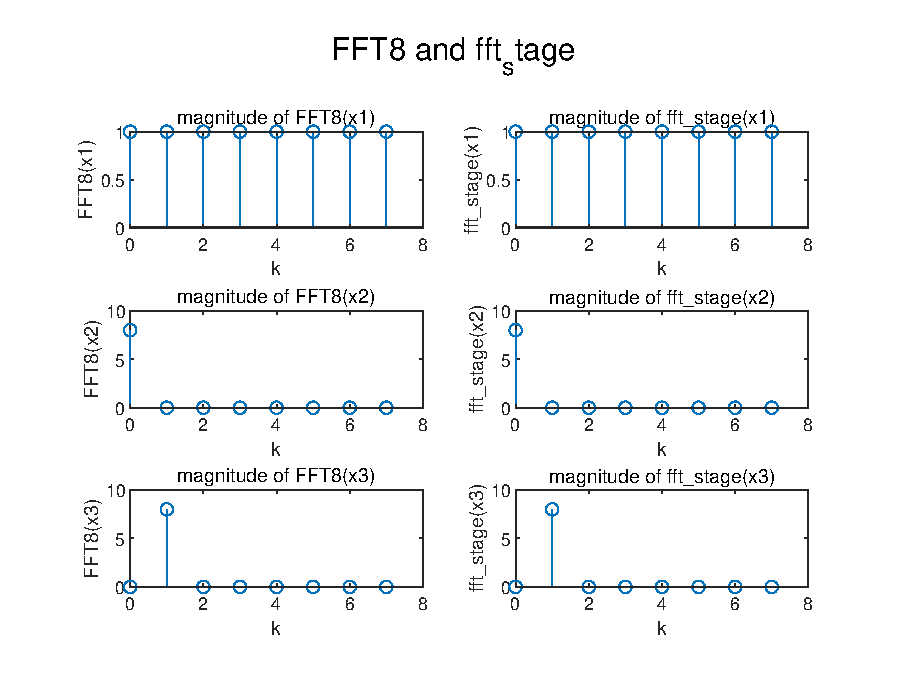
\includegraphics[width=150mm]{pictures/q5_3_2b.eps}
			\caption{Comparison between results obtain from \textbf{fft\_stage.m} and \textbf{FFT8.m}}
		\end{figure}
	\end{itemize}
\end{itemize}

\section*{5.4 My explorations for FFT algorithm}
\begin{itemize}
	\item In the section 5.3.2, FFT algorithm of $N=2^p$ was proposed. But when it comes to the case of  $N\neq 2^{p}$, what
	should we do?\par
	Actually, function fft() in MATLAB just use DFTsum algorithm to calculate it directly. It is inefficient when N is a really large number.
	What we should is to choose the nearestpower-of-two FFT algorithm for implementing a DFT by zero-padding a sequence into an N-point. The 
	idea of zero-padding is shown below:
	\begin{algorithm}[H]
		\caption{Fast Fourier Transform fft\_stage($\mathbf{x}$)}
		\label{alg2}
		\begin{algorithmic}
		\ENSURE $N=\text{length}(\mathbf{x})$
		\IF{$N = 2^p$}
		\IF{$N = 2$}
		\STATE do $2-$pt DFT
		\ELSE
		\STATE calling fft\_stage to compute the ($N/2$)-point DFTs
		\ENDIF
		\ELSE
		\STATE $\mathbf{x} = \text{zero-padding}(\mathbf{x})$
		\STATE $\text{fft\_stage}(\mathbf{x})$
		\ENDIF
	 	\end{algorithmic}
	\end{algorithm}
	\item After searching the Internet, I choose a famous zero-padding operation for OFDM and implement the MATLAB code below:
\begin{lstlisting}[title=\textbf{fft\_stagep.m}]
	function X = fft_stagep(x)
	N = length(x);  
	if log2(N) == fix(log2(N))  % N = 2^m
		if N == 2
			X(1) = x(1)+x(2);
			X(2) = x(1)-x(2);
		else
			r = 0:2:N-1;
			xeven = x(1:2:N);
			xodd = x(2:2:N);
			X0 = fft_stage(xeven);
			X1 = fft_stage(xodd);
			temp = X1.*exp(-j*2*pi/N*r);
			X = [X0+temp X0-temp]; 
		end
	else  % N ~= 2^m
		Nzeros = 2^(fix(log2(N))+1)-N-1;
		x = [x(1:fix(N/2)) zeros(1,Nzeros) x(fix(N/2)+1:N)]; % insert null tones;
		x = [0 x]; % DC subcarrier
		X = fft_stagep(x);      
	end
	end
\end{lstlisting}
\end{itemize}
\newpage
\section*{5.5 Summary \& Experience}
\begin{itemize}
	\item In this lab, we mainly discuss two things:
	\begin{itemize}
		\item The relationship between the DFT and DTFT: DFT is the frequency sampling of DTFT.
		\item Using the method of divide and conquer to recursively implement the Fast Fourier Transform (FFT), which could
		lead a change of number of multiplications from $O(N^2)$ to $O(N\log_2N)$.
	\end{itemize}
	\item All these efforts makes me have a deeper understanding to the principle of DFT and FFT, especially the part of FFT algorithm design.
	\item For the further explorations for FFT algorithm, we can focus more on the zero-padding of FFT.
\end{itemize}
\begin{center}
	\section*{Appendix}
\begin{lstlisting}[title=DFTsum.m]
	function X = DFTsum(x)
	% X_N[k]=\sum_{n=0}^{N-1}x[n]e^{-j*2*pik*n/N}
	% X(k)=\sum_{n=1}^Nx(n)e^(-j*2*pi*(k-1)*(n-1)/N), 1≤k≤N
	N = length(x);
	X = zeros(1,N);
	for k=1:N
	for n=1:N
		X(k)= X(k)+x(n)*exp(-j*2*pi*(k-1)*(n-1)/N);
	end
	end
	end
\end{lstlisting}	
\end{center}

\end{document}